% QFun paper — compile with: pdflatex → bibtex → pdflatex → pdflatex
\documentclass[11pt]{article}

% ---------- packages ----------
\usepackage[margin=1in]{geometry}
\usepackage{amsmath, amssymb, amsfonts, amsthm}
\usepackage{mathtools}
\usepackage{graphicx}
\usepackage{booktabs}
\usepackage{hyperref}
\usepackage{microtype}
\usepackage[numbers,sort&compress]{natbib}
\usepackage{algorithm}
\usepackage{algpseudocode}
\usepackage{bm}
\usepackage{longtable}
\usepackage{array}

% ---------- theorem environments ----------
\newtheorem{definition}{Definition}
\newtheorem{proposition}{Proposition}
\newtheorem{remark}{Remark}

% ---------- convenience macros ----------
\newcommand{\ket}[1]{|#1\rangle}
\newcommand{\bra}[1]{\langle#1|}
\newcommand{\braket}[2]{\langle#1|#2\rangle}
\newcommand{\norm}[1]{\|#1\|}
\newcommand{\abs}[1]{|#1|}
\newcommand{\R}{\mathbb{R}}
\newcommand{\E}{\mathbb{E}}
\newcommand{\calH}{\mathcal{H}}
\DeclareMathOperator*{\argmax}{arg\,max}
\DeclareMathOperator*{\sgn}{sgn}

% ---------- title ----------
\title{\textbf{QFun: Quantum Function Encoding\\with Signed and Quasi-Probability Extensions}}
\author{Kooshan Maleki Dizadji}
\date{\today}

\begin{document}
\maketitle

% ===================================================================
\begin{abstract}
Quantum amplitude encoding embeds a classical vector of $N=2^n$
real numbers into the probability amplitudes of an $n$-qubit state,
achieving an exponential compression of classical data into Hilbert
space.  A fundamental constraint is that measurement obeys the Born
rule, so the observable distribution $p(i)=|\alpha_i|^2$ is always
nonnegative.  This paper presents \emph{QFun}, an open-source
simulation library that implements three layers of amplitude encoding:
(i)~standard nonnegative encoding for one-dimensional and
$d$-dimensional functions on tensor-product grids,
(ii)~\emph{Mode~A}, an ancilla-based scheme that encodes the sign of
each function value into an auxiliary qubit, and
(iii)~\emph{Mode~B}, a two-channel quasi-probability decomposition
that splits a signed distribution into two proper distributions and
recombines them classically.  Mode~B is motivated by the theory of
negative probabilities developed by Dirac, Feynman, Bartlett, and
recently revisited by Polson and Sokolov.  We provide a rigorous
mathematical framework for each mode, analyse statistical convergence,
and demonstrate the library on the 27-equation Feynman benchmark
dataset from the KAN paper.
\end{abstract}

% ===================================================================
\section{Introduction}
\label{sec:intro}

A central primitive in quantum computing is the ability to load
classical data into a quantum register.  Given a vector
$\bm{v}=(v_0,\ldots,v_{N-1})^{\!\top}\!\in\R^N$ with $N=2^n$, one
defines the \emph{amplitude-encoded} state
\begin{equation}\label{eq:ampstate}
  \ket{\psi_{\bm{v}}}
  = \frac{1}{\norm{\bm{v}}_2}
    \sum_{i=0}^{N-1} v_i \ket{i},
\end{equation}
where $\{\ket{i}\}$ is the computational basis of $n$ qubits.  This
encoding underlies quantum linear-system solvers~\cite{harrow2009hhl},
quantum machine learning kernels, and quantum Monte
Carlo techniques.

The price of exponential compression is that direct measurement of
$\ket{\psi_{\bm{v}}}$ in the computational basis yields outcomes
distributed as $p(i)=|\alpha_i|^2\propto v_i^2$, destroying all sign
information.  For nonnegative data this is acceptable: sampling from
$p$ recovers the \emph{shape} of $\bm{v}$.  For signed data the
situation is more subtle and requires additional structure, either in
the quantum circuit or in classical post-processing.

This paper describes \textbf{QFun}, a lightweight, CPU-only Python
library built on PennyLane~\cite{bergholm2020pennylane} that
implements:
\begin{enumerate}
  \item \textbf{Standard amplitude encoding} for nonnegative functions
        on 1D and $d$-dimensional grids
        (Sections~\ref{sec:1d}--\ref{sec:nd}).
  \item \textbf{Mode~A} --- ancilla-based sign encoding
        (Section~\ref{sec:modeA}).
  \item \textbf{Mode~B} --- two-channel quasi-probability
        decomposition (Section~\ref{sec:modeB}), grounded in the
        framework of Polson and
        Sokolov~\cite{polson2024negative}.
  \item The \textbf{Feynman benchmark dataset} of 27 physics
        equations from the KAN paper~\cite{liu2024kan}, originally
        curated by AI~Feynman~\cite{udrescu2020aifeynman}
        (Section~\ref{sec:feynman}).
\end{enumerate}

% ===================================================================
\section{Mathematical Framework}
\label{sec:math}

We develop the formalism in increasing generality: first for a single
real variable, then for multivariate functions on tensor-product grids,
and finally for signed targets.

% -------------------------------------------------------------------
\subsection{Standard amplitude encoding in one dimension}
\label{sec:1d}

\begin{definition}[1D grid]\label{def:grid1d}
Let $f:[a,b]\to\R_{\ge 0}$ be a nonnegative function and let
$n\in\mathbb{N}$ be the number of qubits.  Define $N=2^n$ and the
\emph{uniform grid}
\begin{equation}\label{eq:grid}
  x_i = a + i\,\Delta x,\quad i=0,1,\ldots,N-1,
  \qquad \Delta x = \frac{b-a}{N-1}.
\end{equation}
\end{definition}

Each grid index $i$ has a unique $n$-bit binary representation and
therefore corresponds one-to-one with the computational basis state
$\ket{i}$ of the $n$-qubit Hilbert space
$\calH = (\mathbb{C}^{2})^{\otimes n}$.

\begin{definition}[Amplitude vector]\label{def:amps}
The \emph{raw amplitude} at grid point $x_i$ is
\begin{equation}\label{eq:raw_amp}
  \tilde{\alpha}_i = \sqrt{f(x_i) + \varepsilon},
\end{equation}
where $\varepsilon>0$ is a small regulariser (default $10^{-12}$)
that avoids numerical issues when $f(x_i)=0$.  The \emph{normalised
amplitude vector} is
\begin{equation}\label{eq:norm_amp}
  \alpha_i = \frac{\tilde{\alpha}_i}{\norm{\tilde{\bm\alpha}}_2},
  \qquad
  \norm{\tilde{\bm\alpha}}_2
  = \biggl(\sum_{j=0}^{N-1} \tilde{\alpha}_j^{\,2}\biggr)^{1/2},
\end{equation}
so that $\sum_i |\alpha_i|^2 = 1$.
\end{definition}

\begin{proposition}[Sampling reproduces $f$]\label{prop:born}
Let $\ket{\psi}=\sum_{i}\alpha_i\ket{i}$ be the state prepared by
PennyLane's \texttt{AmplitudeEmbedding}.  By the Born rule, a
computational-basis measurement returns outcome $i$ with probability
\begin{equation}\label{eq:born}
  p(i) = |\alpha_i|^2
  = \frac{f(x_i)+\varepsilon}
         {\sum_{j=0}^{N-1}\bigl(f(x_j)+\varepsilon\bigr)}
  \;\xrightarrow{\varepsilon\to 0}\;
  \frac{f(x_i)}{\sum_j f(x_j)}.
\end{equation}
Hence the empirical histogram of $S$ independent shots converges to a
distribution proportional to $f$ evaluated on the grid.
\end{proposition}

\begin{remark}[Statistical convergence]\label{rem:shots}
If $\hat{p}(i)=c_i/S$ is the relative frequency of outcome $i$ in
$S$ shots (where $c_i$ is the count for outcome $i$), then
$\E[\hat{p}(i)]=p(i)$ and
$\mathrm{Var}[\hat{p}(i)]=p(i)(1-p(i))/S$.  The expected total
$L_1$ error satisfies
$\E\bigl[\sum_i|\hat{p}(i)-p(i)|\bigr] = O\!\left(\sqrt{N/S}\right)$
by Cauchy--Schwarz and the multinomial variance identity.
\end{remark}

\begin{remark}[Interpreting bitstrings]
A measurement outcome such as \texttt{001101} is the binary
representation of an integer index $i$.  QFun converts
$i\mapsto x_i$ via Eq.~\eqref{eq:grid} so that the histogram can be
plotted against the original domain $[a,b]$.
\end{remark}

Figure~\ref{fig:1d_examples} illustrates the 1D encoding for three
nonnegative functions: $f(x)=x^2$, $f(x)=e^{-x^2}$, and
$f(x)=|x|$.  In each panel the red curve is the target distribution
$|\alpha|^2$ and the blue bars are the empirical histogram from
$10^5$ shots on a 6-qubit ($N=64$) grid.

\begin{figure}[t]
  \centering
  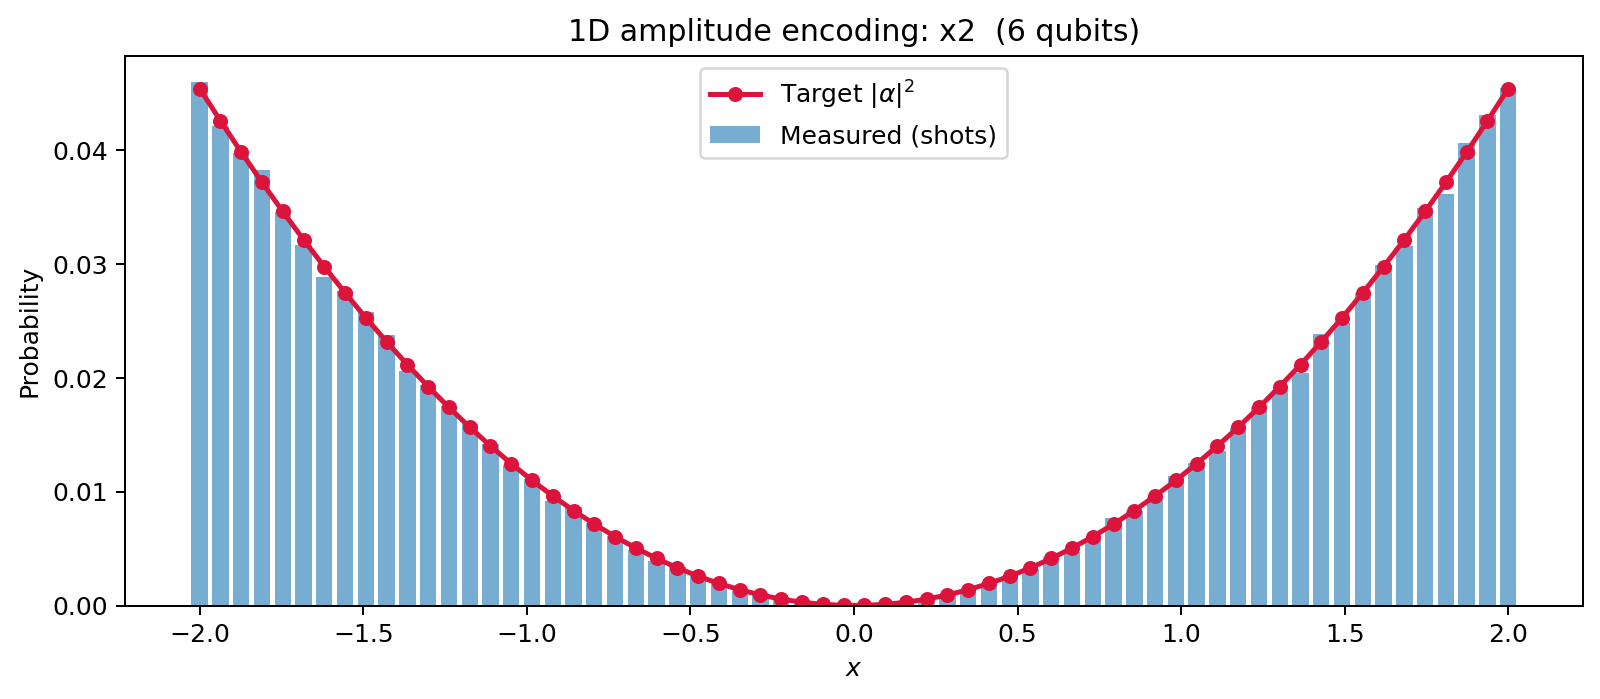
\includegraphics[width=0.95\linewidth]{figures/1D_x2.png}
  \vspace{0.4em}
  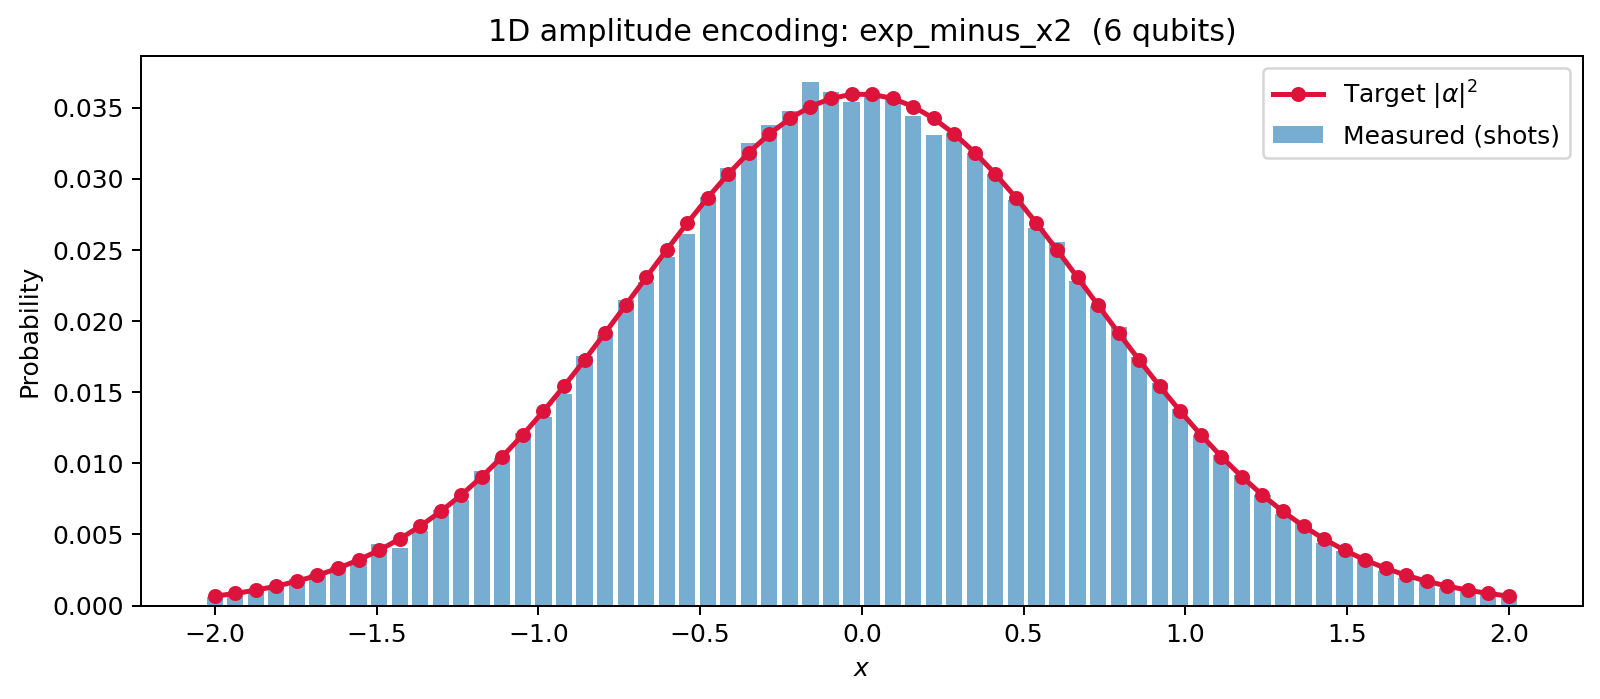
\includegraphics[width=0.95\linewidth]{figures/1D_exp_minus_x2.png}
  \vspace{0.4em}
  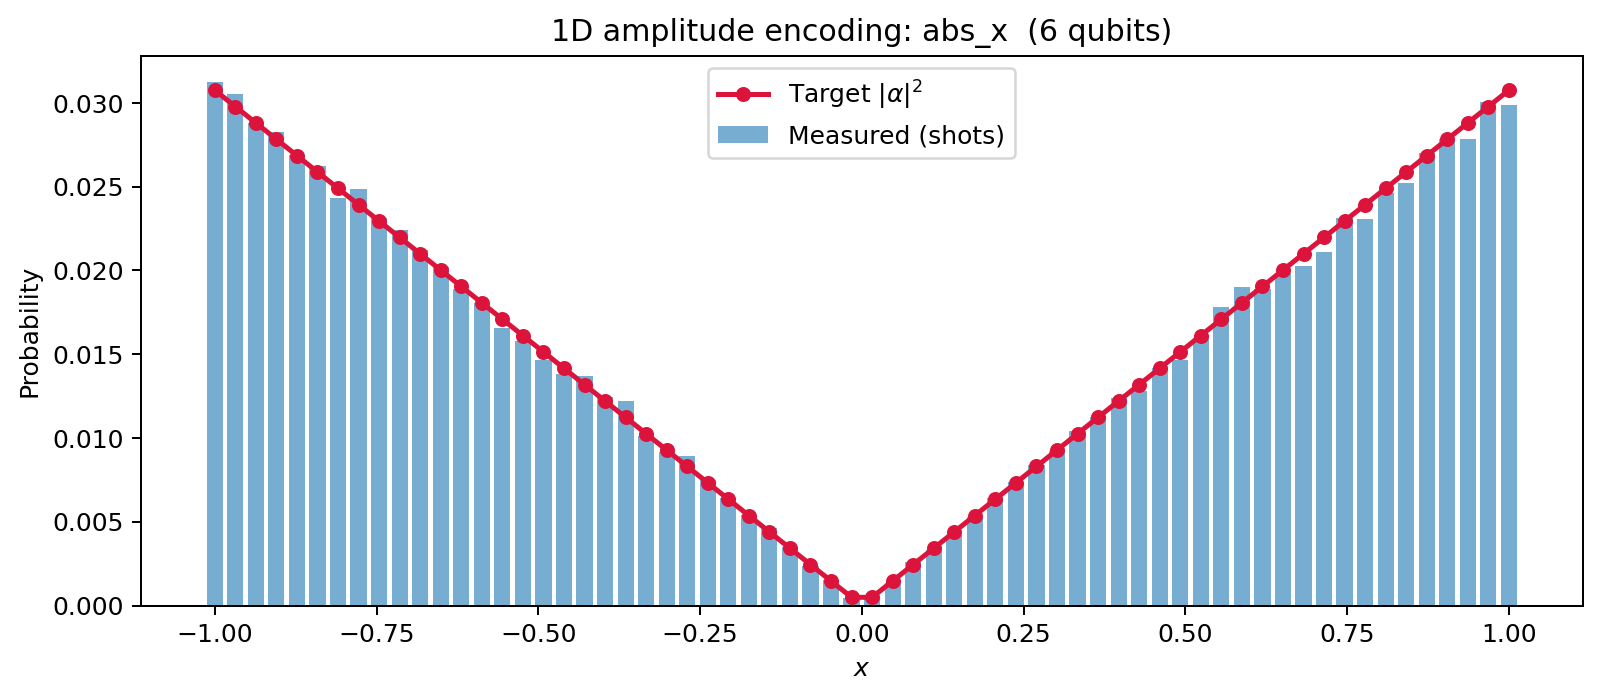
\includegraphics[width=0.95\linewidth]{figures/1D_abs_x.png}
  \caption{Standard 1D amplitude encoding for three nonnegative
  functions on a 6-qubit grid ($N=64$ points, $10^5$ shots).
  Red~curve: target $|\alpha|^2$; blue~bars: measured histogram.}
  \label{fig:1d_examples}
\end{figure}

% -------------------------------------------------------------------
\subsection{Extension to multivariate functions}
\label{sec:nd}

\begin{definition}[Tensor-product grid]\label{def:ndgrid}
For a $d$-variable function $f(x_1,\ldots,x_d)$, allocate $n_k$
qubits to variable $x_k$ with domain $[a_k,b_k]$, $k=1,\ldots,d$.
The 1D grids are
\[
  x_k^{(j_k)} = a_k + j_k\,\Delta x_k,\quad
  j_k=0,\ldots,2^{n_k}-1.
\]
The \emph{tensor-product grid} is the Cartesian product of these 1D
grids, containing
\begin{equation}\label{eq:Nnd}
  N = 2^{n_1+n_2+\cdots+n_d}
\end{equation}
points.  QFun orders them in row-major (C-order) and stores them as a
matrix $\bm{X}\in\R^{N\times d}$.  The total qubit count is
$n = n_1+\cdots+n_d$.
\end{definition}

\begin{remark}[Asymmetric qubit budgets]
Different variables may receive different qubit allocations.  For
example, one may assign $n_1=4$ qubits to a variable with fine
structure and $n_2=3$ to a smoother variable, yielding a $16\times 8$
grid on $n=7$ qubits.
\end{remark}

Function values on the tensor-product grid are flattened to a
length-$N$ vector and amplitude-encoded exactly as in
Section~\ref{sec:1d}.  The existing \texttt{run\_shots} and
\texttt{counts\_to\_distribution} routines therefore work without
modification; only the grid construction and the mapping from flat
index to multi-dimensional coordinates change.

Figure~\ref{fig:I_12_11} shows a 2D example using Feynman equation
I.12.11: $f(a,\theta)=1+a\sin\theta$.

\begin{figure}[t]
  \centering
  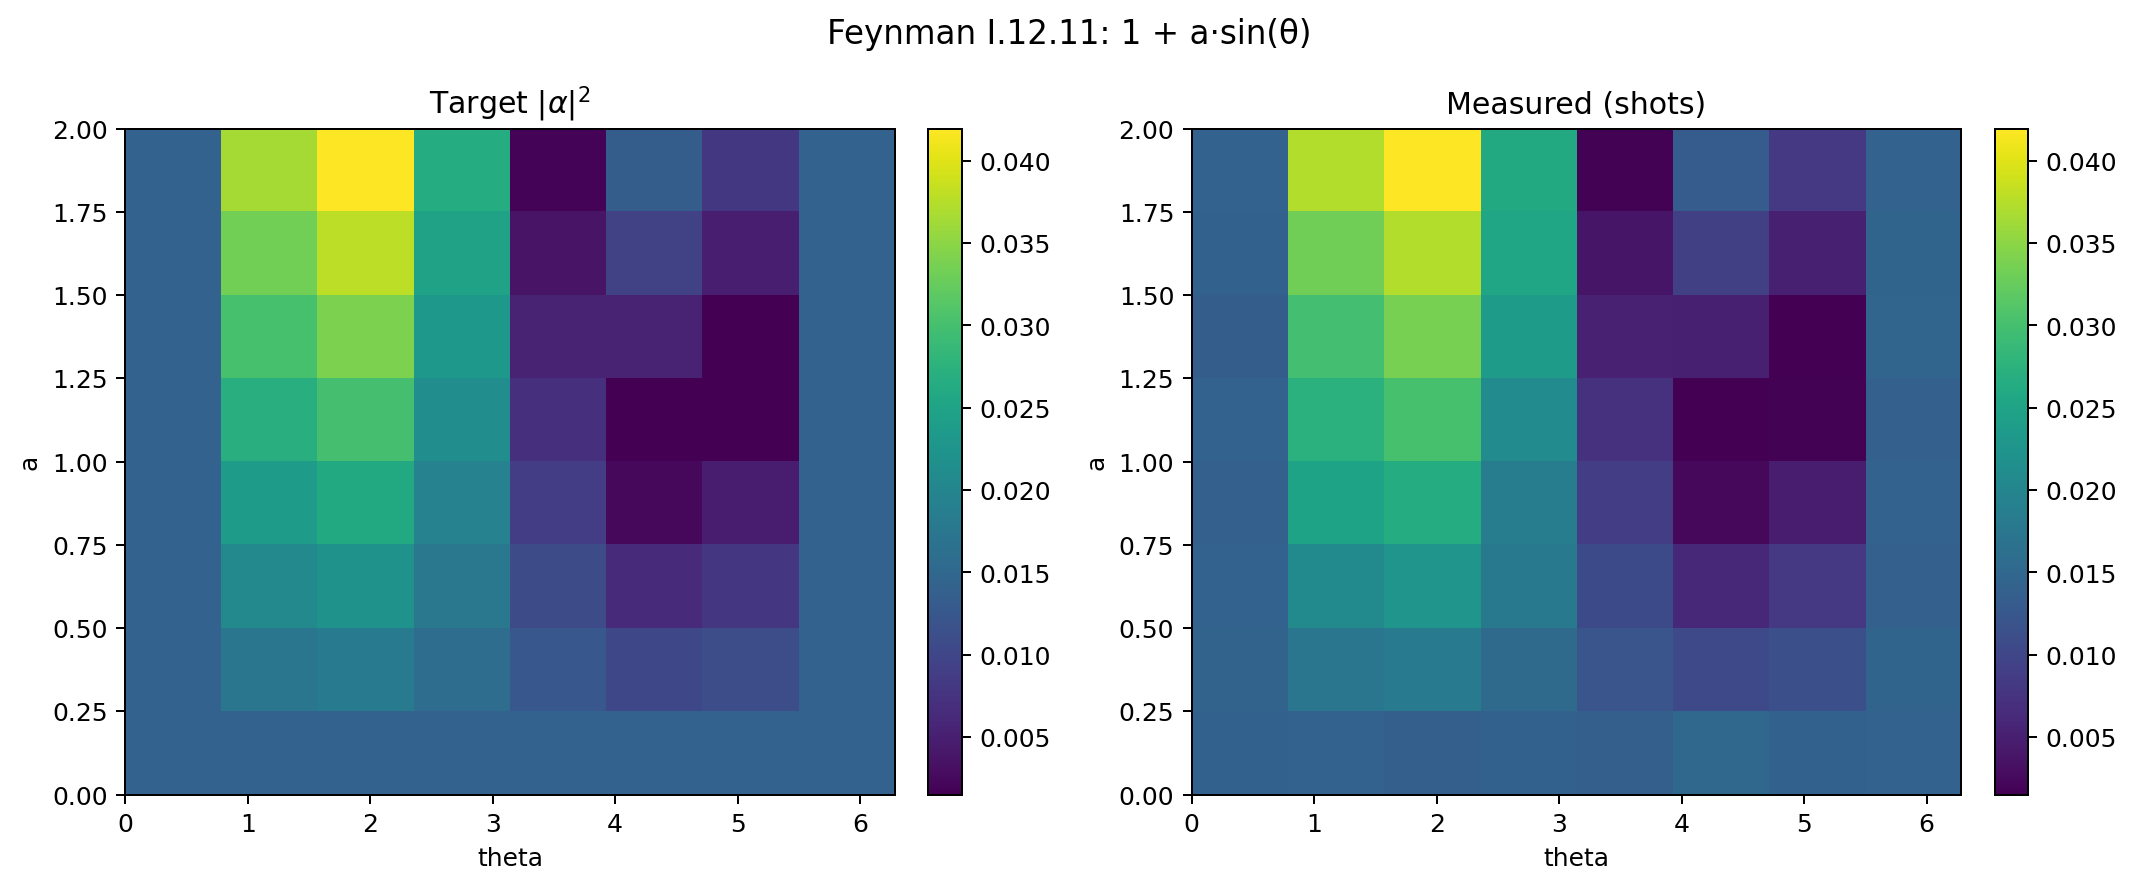
\includegraphics[width=\linewidth]{figures/I_12_11_target_vs_measured.png}
  \caption{2D amplitude encoding for Feynman I.12.11
  ($f(a,\theta)=1+a\sin\theta$) on a $8\times 8$ grid (6 qubits,
  $10^5$ shots).  Left: target $|\alpha|^2$.
  Right: empirical distribution.}
  \label{fig:I_12_11}
\end{figure}

% -------------------------------------------------------------------
\subsection{The negativity problem}
\label{sec:negativity}

If $f(x_i)<0$ for some grid points, the square-root mapping
$\tilde\alpha_i=\sqrt{f(x_i)}$ produces imaginary values, and in any
case $|\alpha_i|^2=|f(x_i)|$ discards the sign.  We therefore
cannot directly recover signed targets from Born-rule measurements
alone.

Historically, the idea that probabilities can be negative appears in
Dirac's work on quantum electrodynamics (1942), Wigner's phase-space
function (1932), and Feynman's discussion of negative probabilities
(1987).  Bartlett~\cite{bartlett1945negative} formulated the key
consistency condition: \emph{negative probabilities must always be
combined with positive probabilities to yield a proper (nonneg)
probability distribution before any physical interpretation is
admissible}.  Polson and Sokolov~\cite{polson2024negative} recently
recast these ideas in a modern statistical framework of
\emph{extraordinary random variables}.  QFun implements two
complementary approaches motivated by this line of work.

% -------------------------------------------------------------------
\subsection{Mode A: ancilla-based sign encoding}
\label{sec:modeA}

The first strategy attaches a single \emph{ancilla qubit} to the data
register to record the sign of each grid value.

\begin{definition}[Signed amplitude state]\label{def:signed_state}
Let $f$ be a real-valued function on the grid and define the
\emph{sign mask}
\begin{equation}\label{eq:signmask}
  b_i =
  \begin{cases}
    0 & \text{if } f(x_i)\ge 0,\\
    1 & \text{if } f(x_i) < 0.
  \end{cases}
\end{equation}
The \emph{magnitude amplitudes} are
$\alpha_i \propto \sqrt{|f(x_i)|+\varepsilon}$, normalised so that
$\sum_i|\alpha_i|^2=1$.  The \emph{signed amplitude state} on
$n+1$ qubits is
\begin{equation}\label{eq:signed_state}
  \ket{\Psi}
  = \sum_{i=0}^{N-1} \alpha_i \ket{i}\ket{b_i}
  \;\in\;
  (\mathbb{C}^{2})^{\otimes(n+1)},
\end{equation}
where the ancilla qubit $\ket{b_i}$ is the least-significant bit.
\end{definition}

\begin{proposition}[Signed reconstruction]\label{prop:signed_recon}
Each computational-basis measurement of $\ket{\Psi}$ yields an
$(n+1)$-bit string whose last bit is the sign bit $b$.
Define the \emph{conditioned empirical distributions}
\begin{equation}\label{eq:ppm}
  \hat{p}_+(i) = \frac{\#\{b=0 \text{ at index } i\}}{S},
  \qquad
  \hat{p}_-(i) = \frac{\#\{b=1 \text{ at index } i\}}{S}.
\end{equation}
Then $\hat{p}_+(i)+\hat{p}_-(i)$ converges to a proper probability
distribution (sums to 1), while the \emph{signed quasi-probability}
\begin{equation}\label{eq:q_modeA}
  \hat{q}(i) = \hat{p}_+(i) - \hat{p}_-(i)
\end{equation}
can take negative values and converges to
$q(i) \propto \sgn(f(x_i))\,|f(x_i)|$ as $S\to\infty$.
\end{proposition}

\begin{proof}
By construction, for each index $i$ the amplitude sits entirely at
$\ket{i}\ket{0}$ or $\ket{i}\ket{1}$, never both.  Therefore
$p_+(i)=|\alpha_i|^2$ when $f(x_i)\ge 0$ and $p_+(i)=0$ otherwise,
with $p_-$ complementary.  Subtracting gives
$q(i)=\sgn(f(x_i))\,|\alpha_i|^2 \propto f(x_i)$.
\end{proof}

\begin{remark}[Circuit structure]
The circuit uses $n+1$ wires.  The first $n$ wires carry the data
register; the last wire is the ancilla.  PennyLane's
\texttt{AmplitudeEmbedding} prepares the $2N$-dimensional state
vector of Eq.~\eqref{eq:signed_state} in a single operation on the
statevector simulator.
\end{remark}

% -------------------------------------------------------------------
\subsection{Mode B: two-channel quasi-probability decomposition}
\label{sec:modeB}

The second strategy operates at the \emph{distribution} level rather
than the state level.  It is directly motivated by the
\emph{extraordinary random variable} framework of Polson and
Sokolov~\cite{polson2024negative}.

\begin{definition}[Signed distribution and its decomposition]
\label{def:decomp}
Let $q:\{0,\ldots,N-1\}\to\R$ be a signed distribution satisfying
$\sum_i q(i)=1$ with some entries negative.  Define
\begin{equation}\label{eq:qpm}
  q^+(i) = \max\bigl(q(i),\,0\bigr),
  \qquad
  q^-(i) = \max\bigl(-q(i),\,0\bigr).
\end{equation}
Let $Z_+=\sum_i q^+(i)\ge 0$ and $Z_-=\sum_i q^-(i)\ge 0$ (with
$Z_+-Z_-=1$).  The \emph{normalised channels} are
\begin{equation}\label{eq:channels}
  p_+(i) = \frac{q^+(i)}{Z_+},
  \qquad
  p_-(i) = \frac{q^-(i)}{Z_-},
\end{equation}
which are proper (nonneg, normalised) probability distributions.
\end{definition}

\begin{proposition}[Exact reconstruction]\label{prop:recon_B}
The signed distribution is recovered by
\begin{equation}\label{eq:recon_B}
  q(i) = Z_+\,p_+(i) \;-\; Z_-\,p_-(i).
\end{equation}
\end{proposition}
\begin{proof}
$Z_+p_+(i)-Z_-p_-(i) = q^+(i)-q^-(i) = q(i)$.
\end{proof}

\paragraph{Procedure.}
QFun amplitude-encodes $p_+$ and $p_-$ independently:
\begin{enumerate}
  \item Prepare $\ket{\psi_+}$ with amplitudes
        $\alpha_i^{(+)}\propto\sqrt{p_+(i)}$; sample $S$ shots to
        obtain $\hat{p}_+$.
  \item Prepare $\ket{\psi_-}$ with amplitudes
        $\alpha_i^{(-)}\propto\sqrt{p_-(i)}$; sample $S$ shots to
        obtain $\hat{p}_-$.
  \item Classically recombine:
        $\hat{q}(i) = Z_+\hat{p}_+(i) - Z_-\hat{p}_-(i)$.
\end{enumerate}

\begin{proposition}[Signed expectations]\label{prop:expect}
For any observable $g:\{0,\ldots,N-1\}\to\R$,
\begin{equation}\label{eq:expect}
  \E_q[g]
  = Z_+ \sum_i g(i)\,p_+(i)
  \;-\; Z_- \sum_i g(i)\,p_-(i)
  = Z_+\,\E_{p_+}[g] \;-\; Z_-\,\E_{p_-}[g].
\end{equation}
The estimator $\hat\E_q[g] = Z_+\hat\E_{p_+}[g]-Z_-\hat\E_{p_-}[g]$
is unbiased with variance
\begin{equation}\label{eq:expect_var}
  \mathrm{Var}[\hat\E_q[g]]
  = \frac{Z_+^2\,\mathrm{Var}_{p_+}[g]}{S}
  + \frac{Z_-^2\,\mathrm{Var}_{p_-}[g]}{S}.
\end{equation}
\end{proposition}

\begin{remark}[Variance amplification]
When the negative mass $Z_-$ is large relative to $Z_+$, both
channels contribute substantial variance and the effective sample
size shrinks.  This is the quasi-probability analogue of the
\emph{sign problem} in quantum Monte Carlo; it is an inherent cost
of representing negativity via nonnegative
sampling~\cite{polson2024negative}.
\end{remark}

Figure~\ref{fig:I_50_26_signed} demonstrates Mode~A on Feynman
equation I.50.26 ($f(a,o)=\cos a + o\cos^2 a$), which takes negative
values.  The diverging colourmap (red--blue) shows the target signed
quasi-probability on the left and the measured reconstruction on the
right.

\begin{figure}[t]
  \centering
  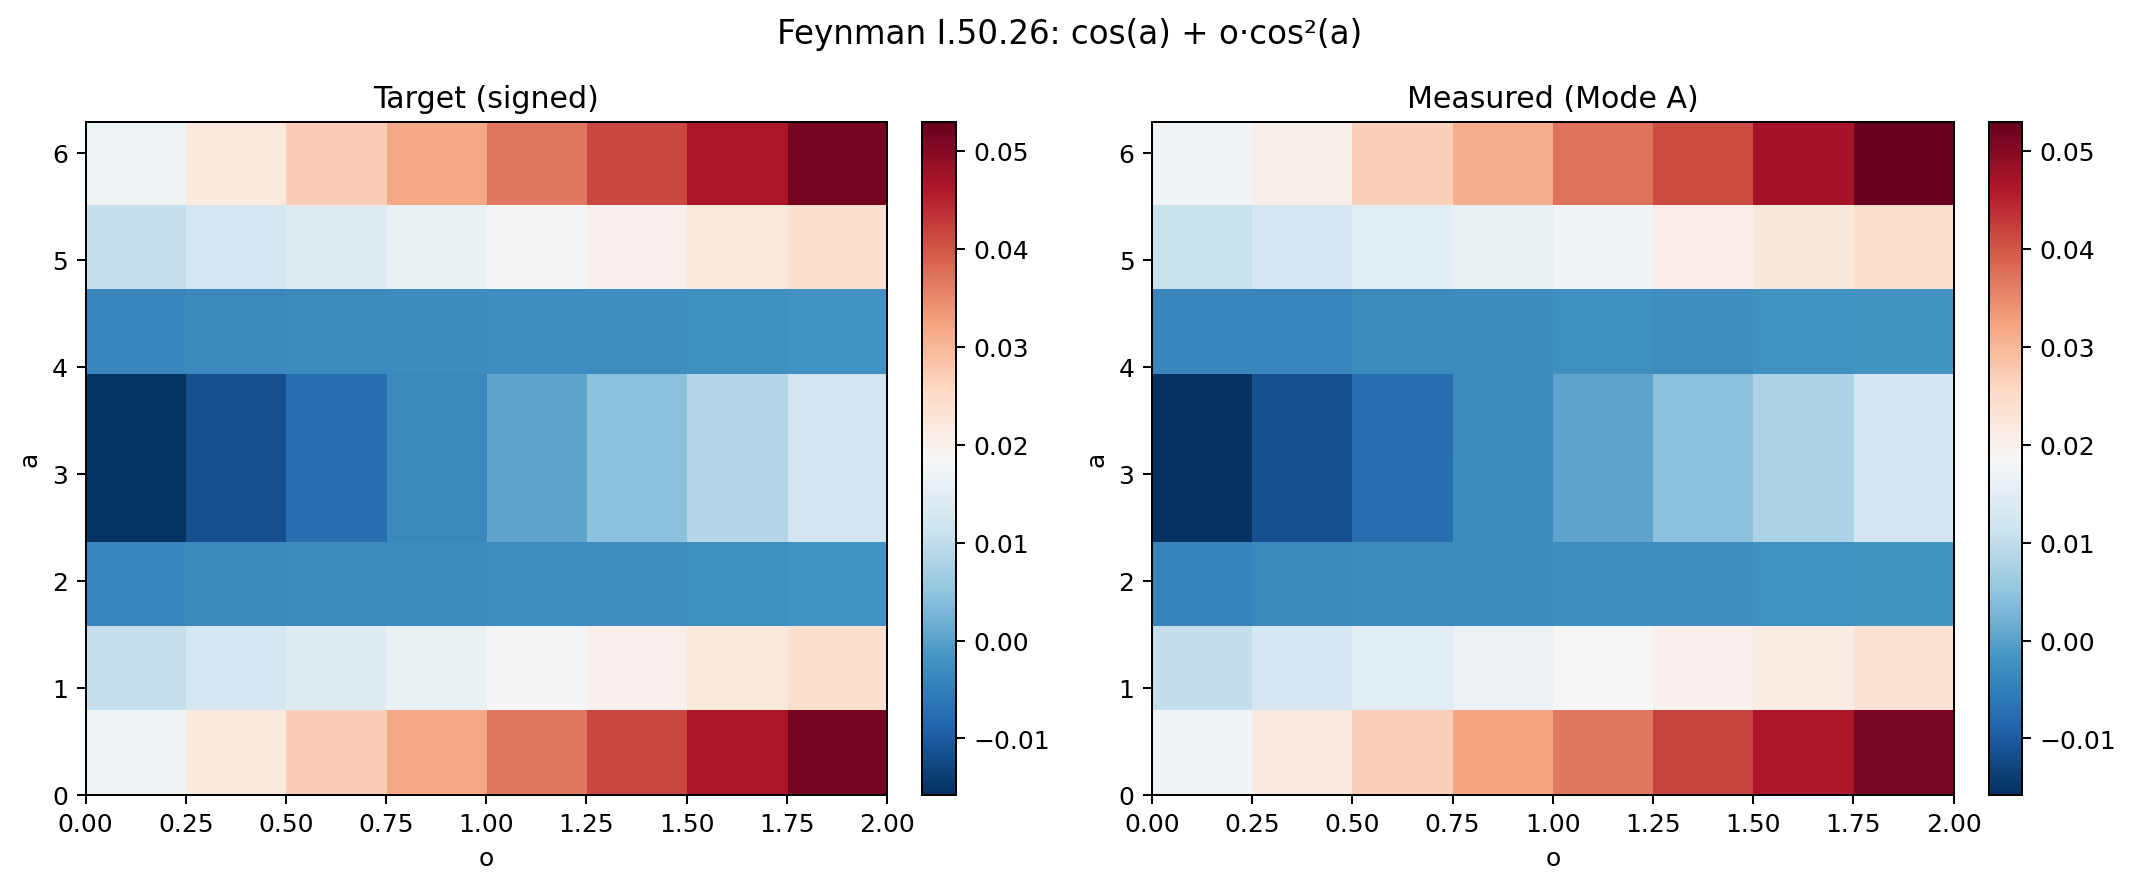
\includegraphics[width=\linewidth]{figures/I_50_26_signed_target_vs_measured.png}
  \caption{Signed (Mode~A) 2D encoding for Feynman I.50.26.
  Left: target signed quasi-probability.
  Right: ancilla-based reconstruction from $10^5$ shots.}
  \label{fig:I_50_26_signed}
\end{figure}

% ===================================================================
\section{Feynman Benchmark Dataset}
\label{sec:feynman}

To facilitate reproducible experiments on multivariate functions, QFun
packages the 27-equation ``Feynman'' benchmark used in the KAN
evaluation table~\cite{liu2024kan} and originally curated for the
AI~Feynman symbolic-regression
challenge~\cite{udrescu2020aifeynman}.

Each equation is stored in its \emph{dimensionless} form (fewer
variables, no physical constants) as a
\texttt{FeynmanEquation} named tuple with the following fields:
\begin{itemize}
  \item \texttt{eq\_id} --- identifier (e.g.\ \texttt{I.12.11}),
  \item \texttt{formula} --- human-readable formula string,
  \item \texttt{variables} --- list of variable names,
  \item \texttt{domains} --- default $[a_k,b_k]$ per variable,
  \item \texttt{func} --- a NumPy-compatible callable.
\end{itemize}
The dataset spans equations with 1 to 6 input variables, covering
Gaussians, trigonometric functions, power laws, and compositions
thereof.  Convenience functions \texttt{list\_equations()} and
\texttt{get\_equation(eq\_id)} provide programmatic access.

Table~\ref{tab:feynman} lists all 27 equations with their
dimensionless formulae, variable counts, and names.

\begin{longtable}{l l c l}
\caption{The 27 Feynman benchmark equations packaged in QFun
(dimensionless forms).}\label{tab:feynman}\\
\toprule
\textbf{ID} & \textbf{Dimensionless formula} & \textbf{\#Vars} & \textbf{Variables} \\
\midrule
\endfirsthead
\toprule
\textbf{ID} & \textbf{Dimensionless formula} & \textbf{\#Vars} & \textbf{Variables} \\
\midrule
\endhead
\midrule
\multicolumn{4}{r}{\emph{continued on next page}} \\
\endfoot
\bottomrule
\endlastfoot
I.6.2     & $\exp(-\theta^2/(2\sigma^2))/\sqrt{2\pi\sigma^2}$ & 2 & $\theta,\;\sigma$ \\
I.6.2b    & $\exp(-(\theta-\theta_1)^2/(2\sigma^2))/\sqrt{2\pi\sigma^2}$ & 3 & $\theta,\;\theta_1,\;\sigma$ \\
I.9.18    & $(a-c)^2+(b-d)^2+(e-f)^2$ & 6 & $a,b,c,d,e,f$ \\
I.12.11   & $1+a\sin\theta$ & 2 & $a,\;\theta$ \\
I.13.12   & $a(1/b-1)$ & 2 & $a,\;b$ \\
I.15.3x   & $a/\sqrt{1-b^2}$ & 2 & $a,\;b$ \\
I.16.6    & $(a+b)/(1+ab)$ & 2 & $a,\;b$ \\
I.18.4    & $(1+ab)/(1+a)$ & 2 & $a,\;b$ \\
I.26.2    & $\arcsin(n\sin\theta_2)$ & 2 & $n,\;\theta_2$ \\
I.27.6    & $1/(1/a+1/b)$ & 2 & $a,\;b$ \\
I.29.16   & $\sqrt{1+a^2-2a\cos(\theta_1-\theta_2)}$ & 3 & $a,\;\theta_1,\;\theta_2$ \\
I.30.3    & $\sin^2(ab/2)/\sin^2(b/2)$ & 2 & $a,\;b$ \\
I.30.5    & $\arcsin(a/b)$ & 2 & $a,\;b$ \\
I.37.4    & $1+a+2\sqrt{a}\cos\delta$ & 2 & $a,\;\delta$ \\
I.40.1    & $n_0\exp(-a)$ & 2 & $n_0,\;a$ \\
I.44.4    & $n\ln a$ & 2 & $n,\;a$ \\
I.50.26   & $\cos a + o\cos^2 a$ & 2 & $a,\;o$ \\
II.2.42   & $(a-1)b$ & 2 & $a,\;b$ \\
II.6.15a  & $(a/c^2)\sqrt{b^2+c^2}$ & 3 & $a,\;b,\;c$ \\
II.11.7   & $n_0(1+p\cos\theta)$ & 3 & $n_0,\;p,\;\theta$ \\
II.11.27  & $a+b$ & 2 & $a,\;b$ \\
II.35.18  & $n_0/(\exp(a)+\exp(-a))$ & 2 & $n_0,\;a$ \\
II.36.38  & $a+ab$ & 2 & $a,\;b$ \\
II.38.3   & $ab$ & 2 & $a,\;b$ \\
III.9.52  & $\sin^2((a-b)c/2)/((a-b)c/2)^2$ & 3 & $a,\;b,\;c$ \\
III.10.19 & $\sqrt{1+a^2+b^2}$ & 2 & $a,\;b$ \\
III.17.37 & $\beta(1+\alpha\cos\theta)$ & 3 & $\beta,\;\alpha,\;\theta$ \\
\end{longtable}

% ===================================================================
\section{Experiments}
\label{sec:experiments}

All experiments use PennyLane's \texttt{default.qubit} statevector
simulator with NumPy as the backend (CPU
only)~\cite{bergholm2020pennylane}.  Figures are reproducible via
\texttt{paper/make\_figures.py}.

\subsection{One-dimensional examples}
Three nonneg functions ($x^2$, $e^{-x^2}$, $|x|$) are encoded on
6-qubit grids and sampled with $10^5$ shots.
Figure~\ref{fig:1d_examples} confirms that the empirical histograms
closely match the target $|\alpha|^2$.

\subsection{Two-dimensional Feynman examples}
We encode Feynman~I.12.11 ($1+a\sin\theta$) on a $8\times 8$ grid
(3 qubits per variable, 6 total) and sample $10^5$ shots.
Figure~\ref{fig:I_12_11} shows the 2D target vs.\ measured heatmaps.

\subsection{Asymmetric qubit budgets}
QFun supports non-uniform qubit allocation across variables.  For
example, encoding Feynman~I.16.6 ($(a+b)/(1+ab)$) with 4 qubits for
$a$ and 3 for $b$ produces a $16\times 8$ grid on 7 total qubits,
giving finer resolution along the variable of interest.

\subsection{Signed multivariate example}
Feynman~I.50.26 ($\cos a + o\cos^2 a$) is negative in part of its
domain.  Mode~A encodes the magnitudes on 6 data qubits plus one
ancilla (7 total).  Figure~\ref{fig:I_50_26_signed} shows the signed
reconstruction from $10^5$ shots.

% ===================================================================
\section{Discussion and Limitations}
\label{sec:discussion}

\paragraph{Exponential grid growth.}
The grid size $N=2^n$ grows exponentially in the number of qubits.
For classical simulation this limits practical demonstrations to
$n\lesssim 20$; on real quantum hardware the limit is set by gate
fidelity and connectivity.

\paragraph{Discretisation error.}
The accuracy with which the sampled distribution represents the
continuous function $f$ depends on both the number of grid points
(resolution) and the choice of domain $[a,b]$.  Functions with sharp
features require more qubits to resolve.

\paragraph{Shot noise.}
As noted in Remark~\ref{rem:shots}, the expected $L_1$ reconstruction
error scales as $O(\sqrt{N/S})$.  For signed estimators (Mode~B),
the effective variance is amplified by a factor of
$\|q\|_1^2 = (Z_++Z_-)^2$ relative to direct sampling
(cf.\ Eq.~\eqref{eq:expect_var}).  Since $Z_+-Z_-=1$, this overhead
equals $(1+2Z_-)^2$ and can be large when the negative mass $Z_-$ is
substantial.

\paragraph{State preparation cost.}
On real hardware, preparing an arbitrary amplitude vector requires
$O(2^n)$ gates in general.  Efficient preparation is an active
research area; QFun uses PennyLane's built-in
\texttt{AmplitudeEmbedding}, which is exact for statevector
simulation.

% ===================================================================
\section{Conclusion}
\label{sec:conclusion}

We presented QFun, a reference implementation of quantum amplitude
encoding for classical functions on 1D and multivariate grids.
Beyond the standard nonneg setting, QFun provides two physically
motivated extensions for signed targets:
\begin{itemize}
  \item \textbf{Mode~A} encodes the sign into an ancilla qubit,
        producing a signed quasi-probability via post-processing.
  \item \textbf{Mode~B} decomposes a signed distribution into two
        proper distributions that are encoded and sampled
        independently, then recombined classically.
\end{itemize}
We also packaged the 27-equation Feynman benchmark for convenient
multivariate demonstrations, and provided a complete mathematical
framework --- including convergence statements and variance
analysis --- for each encoding mode.

% ===================================================================
\bibliographystyle{plainnat}
\bibliography{references}

\end{document}
